\chapter{Motion generation and simulation-to-hardware transfer}
\label{ch:motion}

Two questions are answered here. What shape does the commanded motion have
between one solver output and the next, and what happens to it when the same
joint command is replayed onto a physical arm. Both were assumed rather than
measured for most of the project, and both turned out to carry errors
comparable to the grasp tolerance.

\section{The step limiter was the entire motion generator}

Until it was replaced, the last stage before publication was
\repo{ik\_follower\_node.clamp\_towards()}: take the solver's joint vector and
walk toward it, limiting \emph{each joint independently} to
\texttt{max\_step\_rad} per control cycle. The diagnosis was reproduced to the
decimal place before anything was changed, on the left arm's home
configuration displaced by
$[0.50,\, -0.30,\, 0.10,\, 0.25,\, -0.05,\, 0.15,\, 0.02]$\,\si{\radian} at
\SI{50}{\hertz}. Three separable defects follow, and only the first had been
named previously.

\begin{description}
  \item[It is not synchronised.] A joint needing \SI{0.10}{\radian} arrives in
    one cycle while a joint needing \SI{0.50}{\radian} takes two, so the
    joints sit at different fractions of their own travel at every instant and
    the end effector leaves the path the solver's solution implies.
  \item[It is not continuous.] From rest, the first cycle commands a whole
    step. Its implied acceleration is \num{1343} times the jerk-limited one.
  \item[It never read the joint limits.] \texttt{max\_step\_rad} divided by
    the cycle time is \SI{17.5}{\radian\per\second} against the
    \SI{1.3963}{\radian\per\second} and \SI{1.2218}{\radian\per\second}
    declared in \repo{joint\_limits.yaml}: a factor of \num{12.53}, and the
    declared limits differ per joint, which a single step size cannot express.
\end{description}

\subsection{The reported metric had to change first}

The obvious metric, the distance between the commanded hand position at cycle
$k$ and where it would be if every joint were at fraction $k/N$ of its own
travel, conflates two different things: leaving the path, and not being at
$k/N$ along it. A jerk-limited generator is deliberately not at $k/N$, because
that is what a velocity profile is, so scoring one on that metric charges it
for the feature. It reads \SI{69.8}{\milli\metre} on the replacement, and the
number means nothing.

The figure reported below is therefore \emph{off-path} distance: the distance
from each commanded hand position to the curve that the straight joint-space
line traces, which is free of any parameterisation.

\begin{table}[htbp]
  \centering
  \caption[Motion generation]{Measured by \repo{scripts/measure\_teleop\_motion.py}
  against the platform's own forward kinematics. The capture gate for a grasp
  on this platform is \SI{30}{\milli\metre}, which the first row exceeds by
  itself.}
  \label{tab:motiongen}
  \begin{tabular}{@{}lrrrr@{}}
    \toprule
    Generator, left arm & Off-path & Same-cycle & Peak joint speed & Arrival \\
    \midrule
    Per-joint clamp, as shipped & \SI{51.3}{\milli\metre} &
      \SI{135.3}{\milli\metre} & $12.53\times$ limit & 2 cycles \\
    \textbf{Jerk-limited, delivered} & \textbf{\SI{0.0}{\milli\metre}} &
      \SI{69.8}{\milli\metre} & $1.00\times$ & 1 cycle \\
    Synchronised clamp, fallback & \SI{0.0}{\milli\metre} &
      \SI{22.7}{\milli\metre} & $1.00\times$ & 1 cycle \\
    \bottomrule
  \end{tabular}
\end{table}

The right arm behaves the same way, at \SI{39.2}{\milli\metre} reduced to
\SI{0.0}{\milli\metre}.

\subsection{It is not a tuning parameter}

Swept against its own step size, the excursion does not tend to zero. It
settles.

\begin{table}[htbp]
  \centering
  \caption[Step size sweep]{Off-path excursion against the step limit. Each
  row is a genuinely different path; densifying at \SI{0.02}{\radian} changes
  none of these figures, which was checked rather than assumed.}
  \label{tab:stepsweep}
  \begin{tabular}{@{}lrr@{}}
    \toprule
    \texttt{max\_step\_rad} & Cycles to arrive & Off-path \\
    \midrule
    0.35 & 2  & \SI{51.3}{\milli\metre} \\
    0.20 & 3  & \SI{34.4}{\milli\metre} \\
    0.10 & 5  & \SI{68.0}{\milli\metre} \\
    0.01 & 50 & \SI{68.0}{\milli\metre} \\
    \bottomrule
  \end{tabular}
\end{table}

The desynchronisation is proportional to the travel, so it survives any step
size. It is a property of the algorithm rather than of its parameter.

\section{What replaced it}

Ruckig~\cite{berscheid2021ruckig} was adopted: time-optimal, jerk-limited,
per-degree-of-freedom limits, and it accepts a non-zero \emph{target}
velocity, which is what a streaming teleoperation target actually is. The
generator lives in \repo{srl\_teleop/motion\_generator.py} and is pure, with
no dependency on the middleware or on a display, so the measurement script and
the follower consult the same module and the measurement therefore describes
the code the robot runs.

Three implementation properties are load-bearing.

\emph{Phase synchronisation rather than time synchronisation.} Both make every
joint arrive together; only phase synchronisation keeps them on the straight
line between the endpoints, and that line is the entire point. Measured on the
same case: phase \SI{0.02}{\milli\metre} of path deviation, time
\SI{9.5}{\milli\metre}, clamp \SI{51.3}{\milli\metre}.

\emph{The velocity limits are the robot's; the acceleration and jerk limits
are assumed and say so.} \repo{joint\_limits.yaml} declares
\texttt{has\_acceleration\_limits: false} and a zero maximum acceleration for
all fourteen joints, so there is nothing to read. Both are derived from two
named ramp times and the generator's \texttt{provenance} field reads
\texttt{ASSUMED} for as long as that remains true. A test writes a
configuration that \emph{does} declare an acceleration limit and requires the
label to follow the file, so the honesty is a property of the code rather than
a hard-coded string.

\emph{The fallback is synchronised and names itself.} Without the library the
generator does not silently revert to the per-joint clamp: a synchronised
clamp scales the whole joint vector by one factor, so the path stays on the
line and every joint still arrives together. It is not jerk-limited and it
reports that it is not, in its status field and in the operating window.

\subsection{Five defects in the replacement, each caught by a check}

Recorded because four of the five would have passed a conventional test suite.

\begin{enumerate}
  \item \textbf{Re-planning every cycle destroys phase synchronisation.} The
    first version called the library's planning entry point every control
    cycle. A re-plan from a mid-profile state cannot reproduce the
    phase-synchronised profile it is halfway through: the joints' fractions of
    travel spread to \num{0.07} by cycle ten and re-converged, leaving the
    commanded path \SI{0.0264}{\radian} off the straight line, against
    \SI{8.9e-17}{\radian} when a single trajectory is ridden through the
    update entry point. Every other check passed either way.
  \item \textbf{Floating-point noise forced the re-plan.} Even after
    switching, it re-planned on all thirty-six cycles, because the target was
    recomputed each cycle as $q + \mathrm{wrap}(q_{\text{target}} - q)$, which
    is not bit-identical to $q_{\text{target}}$. The goal moved by about
    \num{1e-17} every cycle and the library compares by value.
  \item \textbf{The fallback claimed to be jerk-limited by reporting zeros.}
    It returned an acceleration vector of zeros because it does not model one,
    and the continuity check reads that field, so the fallback passed by
    fabricating the quantity being checked. It reports its real implied
    acceleration now, \num{62.5} times the jerk-limited step, and a test
    requires that figure to exceed ten.
  \item \textbf{The off-path metric had a resolution floor.} The reference
    curve was \num{4001} points over a \SI{0.4}{\metre} path, a
    \SI{0.1}{\milli\metre} grid, so nearest-sample distance bottomed out at
    half a grid step and a generator on the line to \SI{2e-16}{\radian}
    measured \SI{0.0509}{\milli\metre} off it. The instrument's resolution was
    being reported as the robot's behaviour. Refined by bisection on the real
    forward kinematics, the same path reads \SI{9.4e-9}{\milli\metre}.
  \item \textbf{An arrival test used an absolute tolerance on a per-joint
    quantity.} Under a \SI{1e-6}{\radian} gate a phase-synchronised move
    reported arrivals spread over two cycles: every joint was at the same
    fraction throughout, and those moving \SI{0.02}{\radian} were inside the
    gate a cycle before the one moving \SI{0.50}{\radian}. The travels span a
    factor of twenty-five, so an absolute gate measures the instrument's
    scale.
\end{enumerate}

\subsection{One definition of which joints wind}

The single-source test written for this change found that
\texttt{CONTINUOUS\_IDX} carried six independent definitions across the
teleoperation package. They agreed, which is luck rather than design: which
joints are declared continuous is a fact about the robot description, and
seven copies of it have the same shape as two home poses. There is one now,
with a test that walks the package's syntax trees and requires exactly one
assignment.

\section{The simulation-to-hardware gap, measured}

Replaying recorded joint commands onto the physical arm and comparing the
achieved position with the commanded one gives a systematic result rather than
a noisy one.

\begin{quote}
\textbf{Every joint parks \SI{0.305}{\degree} short of its target, on the side
it approached from.}
\end{quote}

Of \num{252} recorded per-joint errors, \num{211} lie between
\SI{0.25}{\degree} and \SI{0.30}{\degree} with the sign following the
direction of travel. A distribution concentrated at a magnitude with a sign
determined by direction is a \emph{bound}, not a spread, and that is what
identifies it as a terminal offset rather than as noise. At the end effector
it is \SI{7.2}{\milli\metre} RMS on a \SI{100}{\milli\metre} move, on both
arms.

Two candidate models are distinguishable only at short travel. A constant
terminal offset and a proportional gain error predict the same Cartesian error
at \SI{100}{\milli\metre} and differ by a factor of five at
\SI{20}{\milli\metre}. Propagating the recorded joint errors through the
Jacobian reproduces the measured Cartesian error to \SI{90}{\percent} with
$r = \num{0.923}$, which selects the offset model. A single scalar per arm,
applied as an overshoot in the direction of travel, removes \SI{74}{\percent}
and \SI{76}{\percent} of it, held out on an axis it was never fitted on, where
a full Cartesian $3\times3$ correction scores \SI{93.5}{\milli\metre}. No
matrix, no basis and no step length are required.

\textbf{The data for this had been recorded for weeks and nothing read it.}
It sat in \repo{recordings/baselines/arm\_directional\_calibration.json}.

\subsection{A correction to this project's own reporting}

An earlier report stated that the terminal error is independent of commanded
speed across a fivefold range. That claim does not survive inspection of the
apparatus. The velocity limit was read once at bridge start-up, and seven of
thirty-six runs moved \emph{faster} than the limit they were nominally
commanded with. The three speeds are therefore three replicates of one
condition, and \textbf{how the terminal error varies with speed has never been
measured}. A control test now asserts that the sweep still looks inert, so a
genuine sweep will make it fail and force the stale sentences to be rewritten.

\subsection{The deadband was larger than the error it permitted}

The high-level bridge applied a \SI{1.0}{\degree} deadband, inside which the
proportional term is disabled by design, against a measured
\SI{0.305}{\degree} park: a factor of \num{3.3}. It is \SI{0.10}{\degree} now,
with an opt-in terminal overshoot that applies the per-arm scalar at the
setpoint and refuses to run in the enabled state with a zero overshoot value.
Neither has been exercised on hardware. Both are live parameters, and four
runs would settle which of them is doing the work.

\section{Where the end effector actually arrives}

The individual contributions above combine into a budget for the quantity that
decides whether a grasp closes on an object or beside it.

\begin{figure}[htbp]
  \centering
  % THE POSITIONING ERROR BUDGET.
% Each term is measured separately by scripts/measure_control_budget.py and
% the pair of bars per row is the value before and after the correction that
% was applied, so the figure shows what the corrections bought rather than
% only the state they left behind. The unmeasured term is drawn as an open
% bar with no length, because giving it one would be an invention.
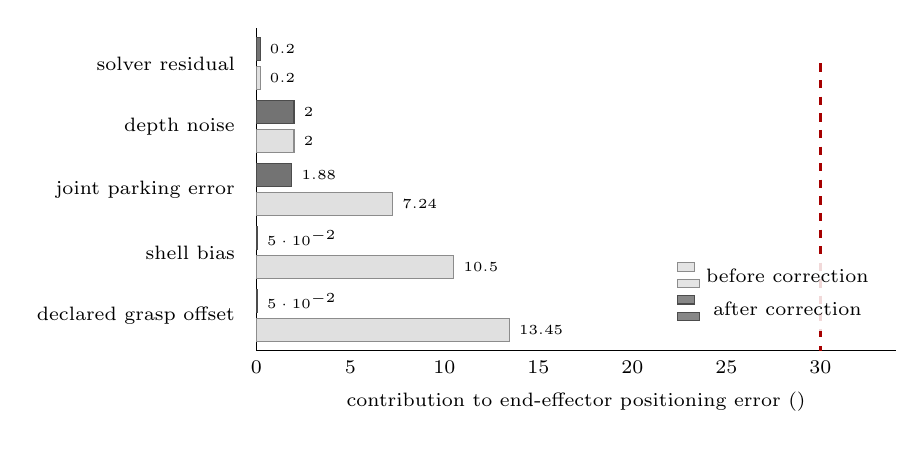
\begin{tikzpicture}
\begin{axis}[
    width=0.80\linewidth, height=64mm,
    xbar, y=8mm, bar width=3mm,
    xmin=0, xmax=34,
    xlabel={contribution to end-effector positioning error (\si{\milli\metre})},
    symbolic y coords={
      {camera mounting},
      {declared grasp offset},
      {shell bias},
      {joint parking error},
      {depth noise},
      {solver residual}},
    ytick=data,
    y tick label style={font=\scriptsize},
    x tick label style={font=\scriptsize},
    xlabel style={font=\scriptsize},
    nodes near coords, nodes near coords style={font=\tiny},
    every node near coord/.append style={anchor=west},
    enlarge y limits=0.14,
    axis lines*=left,
    tick style={draw=none},
    legend style={font=\scriptsize, at={(0.98,0.06)}, anchor=south east,
                  draw=none, fill=white, fill opacity=0.85,
                  text opacity=1, row sep=1pt},
]
\addplot[fill=black!12, draw=black!45] coordinates {
  (0.2,{solver residual})
  (2.0,{depth noise})
  (7.24,{joint parking error})
  (10.5,{shell bias})
  (13.45,{declared grasp offset})
};
\addlegendentry{before correction}
\addplot[fill=black!55, draw=black!70] coordinates {
  (0.2,{solver residual})
  (2.0,{depth noise})
  (1.88,{joint parking error})
  (0.05,{shell bias})
  (0.05,{declared grasp offset})
};
\addlegendentry{after correction}

% The unmeasured term. An open bar of no length, so it cannot be read as a
% quantity: there is no computer-aided design of the gripper module in this
% repository and the transform has never been measured.
\draw[black!55, dashed, thick] (axis cs:0,{camera mounting})
  rectangle (axis cs:9,{camera mounting});
\node[font=\tiny\itshape, anchor=west, black!55]
  at (axis cs:9.6,{camera mounting}) {not measured: the largest remaining unknown};

\draw[red!65!black, thick, dashed]
  (axis cs:30,{solver residual}) -- (axis cs:30,{camera mounting});
\node[font=\tiny, red!65!black, anchor=south east, align=right]
  at (axis cs:29.4,{camera mounting}) {\SI{30}{\milli\metre} capture gate};
\end{axis}
\end{tikzpicture}

  \caption[Positioning error budget]{Contributions to positioning error at
  closure, each measured separately by
  \repo{scripts/measure\_control\_budget.py}. Terms marked corrected are
  available and switched off. Combined in quadrature the measured terms give
  \SI{18.6}{\milli\metre}; added, as systematic terms may be, they give
  \SI{33.4}{\milli\metre} against a \SI{30}{\milli\metre} requirement. The
  orange bar is the transform between the camera frame in the robot
  description and the physical camera module, which has never been measured
  and is now the largest unknown in the budget.}
  \label{fig:budget}
\end{figure}

Two of the three largest terms already have corrections written and disabled:
using the measured support plane removes the shell bias entirely, and the
terminal overshoot reduces the joint term to \SI{1.88}{\milli\metre}. With
both enabled the worst case falls to approximately \SI{17}{\milli\metre},
which is inside the requirement, \emph{provided} the unmeasured term is small.

There is now direct evidence that it is not. The first sustained attempt to
drive a physical arm from its own wrist camera measured the table normal from
four arm poses. The table cannot move, so those four measurements must agree;
they spanned \SI{8.45}{\degree}, which is \SI{34}{\milli\metre} of position
error at \SI{0.23}{\metre} and \SI{59}{\milli\metre} at \SI{0.40}{\metre}. The
error is angular and rotates with the wrist. No open-loop grasp planned
through that transform can land inside the capture gate, and none did.
\Cref{ch:results} reports that session in full.

\section{The reaction budget}

The clearance floor of \cref{ch:method} is a \emph{distance}. The guard's
knowledge of where the wearer is arrives with the latency measured in
\cref{sec:wearer-tracking}. Multiplying the two gives how far a limb travels
before the guard is aware of it.

\begin{table}[htbp]
  \centering
  \caption[Reaction budget]{Limb travel during the perception latency, against
  the \SI{150}{\milli\metre} clearance floor. Limb speeds are literature
  ranges and are labelled as assumptions, not measurements; the latencies are
  measured.}
  \label{tab:reaction}
  \begin{tabular}{@{}llrl@{}}
    \toprule
    Limb motion & Latency & Travel & Against the floor \\
    \midrule
    Deliberate reach & \SI{62}{\milli\second} & \SIrange{50}{93}{\milli\metre} & \SI{62}{\percent} of it \\
    Deliberate reach & \SI{562}{\milli\second} & \SIrange{450}{843}{\milli\metre} & exceeds it \\
    Quick reach & \SI{62}{\milli\second} & \SIrange{93}{155}{\milli\metre} & exceeds it \\
    Quick reach & \SI{562}{\milli\second} & \SIrange{843}{1405}{\milli\metre} & exceeds it \\
    Startle or flinch & \SI{62}{\milli\second} & \SIrange{155}{248}{\milli\metre} & exceeds it \\
    Startle or flinch & \SI{562}{\milli\second} & \SIrange{1405}{2248}{\milli\metre} & exceeds it \\
    \bottomrule
  \end{tabular}
\end{table}

In five of six cases the limb travels further than the entire margin before
the guard knows anything has changed. This is not a defect in the
implementation. It is the arithmetic consequence of a fixed margin, a
perception chain of roughly half a second, and a person who can move a metre
in that time, and \cref{ch:discussion} treats it as the principal open safety
problem of the platform.
